\section*{Abstrakt} 
\addcontentsline{toc}{section}{Abstrakt} 
\vspace{1em}

This report documents the design and implementation of an arcade inspired "endless runner" game, developed for the ARM Cortex-M4 CPU microcontroller using the STM32CubeIDE. The project emphasizes a modular software architecture, structured into the distinct layers: the Application Layer, the Application Interface Layer and the Hardware Abstraction Layer (HAL). This layerd appoach ensures code portability and maintainability by isolation hardware-specific drivers from the core game logic.

The game features an evolving difficulty system where gamplay speed and the players hitbox size increases over time. Technical implementation includes the use of fixed-point arithmetic for efficient physics calculations in a resource-constrained environment, as well as hardware timers (TIM2) to maintain a stable 30 Hz update frequency. Player-interaction is handled through a joystick and buttons, with visual feedback provided via an SPI-driven LCD and an RGB LED.

Key game mechanics such as collision detection, randomized projectile trajectories, and various power-ups (shields, score multipliers, and extra lives) were successfully integrated. The project demonstrates the successful synthesis of low-level hardware control and high-level software design, fulfilling the requirements for the 30010 Programming Project.

\vspace{15em}

\begin{figure}[h]
    \centering
    \begin{subfigure}{0.35\textwidth}
        
\includegraphics[width=\linewidth]{Picturs/signaturs/safija.jpeg}
        \caption{Safija Aagerup}
    \end{subfigure}
    \begin{subfigure}{0.42\textwidth}
        
\includegraphics[width=\linewidth]{Picturs/signaturs/image.png}
        \caption{William Riss}
    \end{subfigure}
\end{figure}

\begin{figure}[h]
    \centering
    \begin{subfigure}{0.45\textwidth}
        
\includegraphics[width=\linewidth]{Picturs/signaturs/nymand.png}
        \caption{Nikolaij Nymand}
    \end{subfigure}
    \begin{subfigure}{0.30\textwidth}
        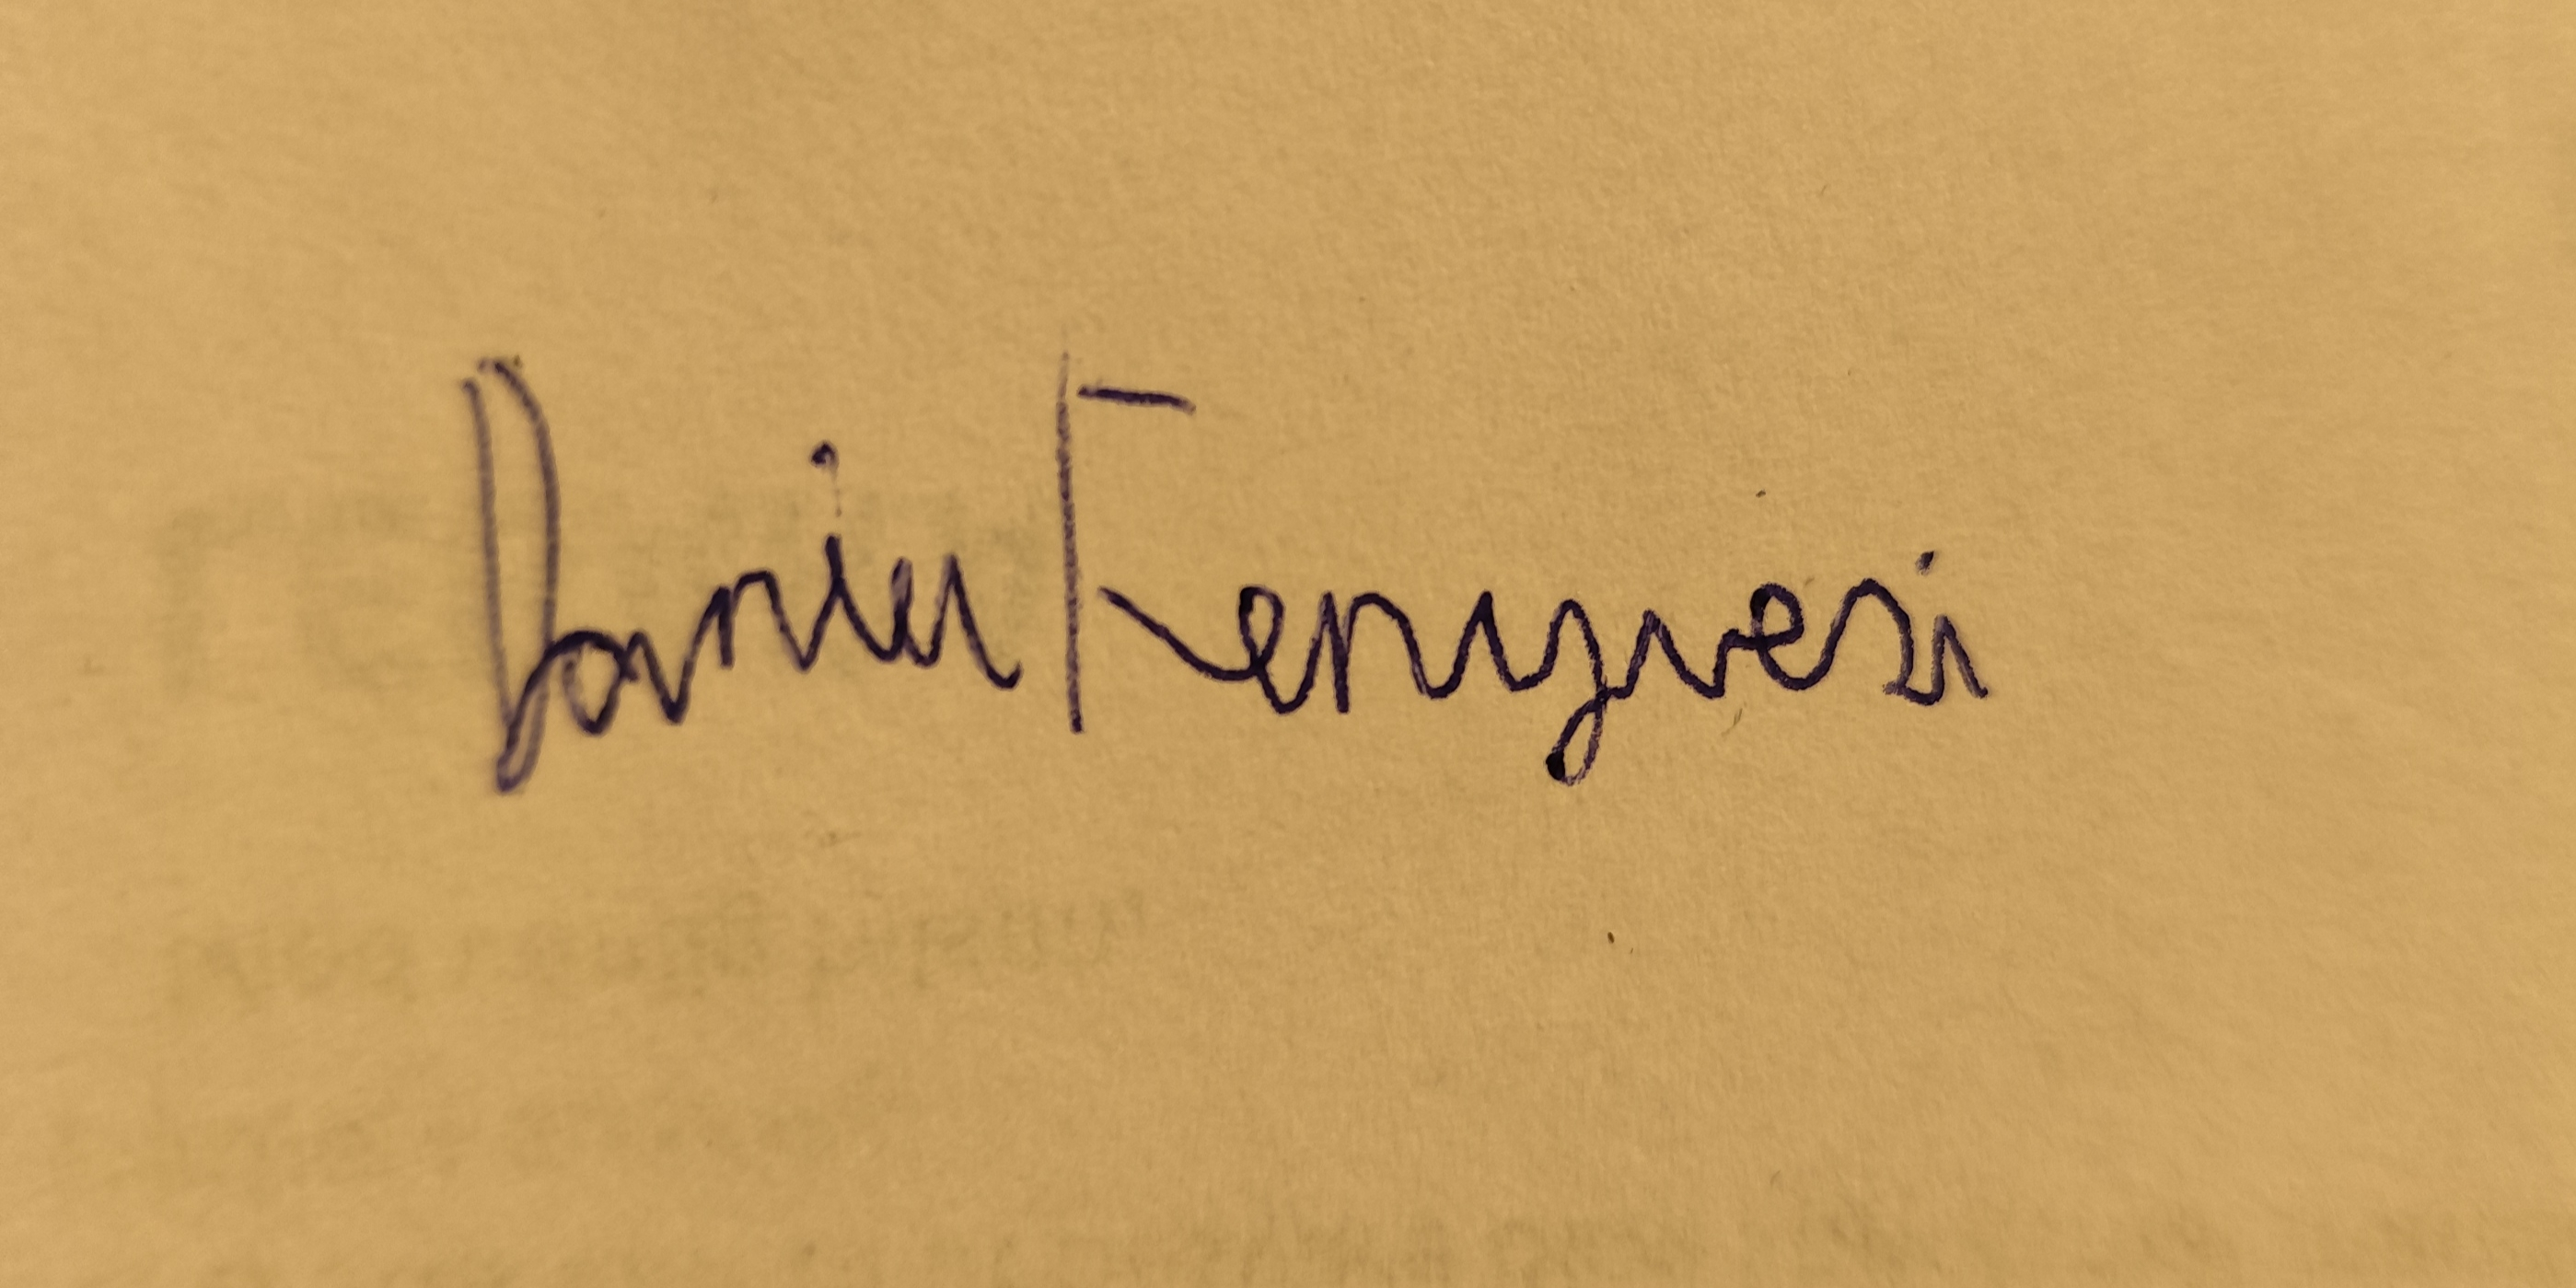
\includegraphics[width=\linewidth]{Picturs/signaturs/Daniel.jpg}
        \caption{Daniel Fenyvesi}
    \end{subfigure}
\end{figure}




\clearpage
\section*{Resume} 
\addcontentsline{toc}{section}{Resume} 
\vspace{1em}

Dette projekt dokumentere udviklingen at et funktionnelt arkadespil. Gennem projektet er der lagt vægt på at skabe en robust softwarearkitektur, der adskiller spil logik fra hardwarehåndtering, via en trelags model (application, Interface og HAL).

Det færdige system understøtter dynamisk sværhedsgrad og udnytter teknikker som fixed-point aritmetik og hardwaretimere for at opnå en stabil opdateringsfrekvens på 30 Hz, på trods af mikrocontrollerens begrænsede ressourcer. Spillet integrerer fuldt ud relevante perifere enheder, herunder joystick, LCD-display og RGB-LED.

Projektet demonstrerer en praktisk anvendelse af centrale elementer fra kursus 30010, såsom kollisionsdetektering, interrupt-håndtering og modulær programmering i C. Samlet set resulterer dette i et stabilt, udvideligt og veldokumenteret system, der lever op til samtlige opstillede designkrav.


